\documentclass{beamer}
\setbeamertemplate{navigation symbols}{}
\usepackage{beamerthemeshadow}
\usepackage{amsmath}
\begin{document}

\title[Dashboard for MAB Algorithms]{Dashboard for Multi Armed Bandit (MAB) Algorithms}
\author[Surbhi Gupta, Kishan Patel]{Surbhi Gupta, Kishan Patel}
\date{November 13, 2013}

\begin{frame}
\titlepage
\begin{center}
Supervisor: Aditya Mahajan, Design Project 1
\end{center}
\end{frame}

\begin{frame}
\tableofcontents
\end{frame}

\section{Overview}

\subsection{Objective and Purpose}
\begin{frame}{Objective and Purpose}
\textbf{Objective}
\newline To represent the results of executing a generic class of
MAB algorithms used for Website Optimization (WO)
\newline
\\\textbf{Purpose}
\\Ease of identification of best performing (most efficient) MAB algorithm for WO as well as
\begin{itemize}
  \item In-depth visual understanding
  \item Engaging interactive design
\end{itemize}
\end{frame}

\subsection{Terminology}
\begin{frame}{Terminology}
Some terms to familiarize with 
\begin{itemize}
  \item \textbf{Agent}: Decision maker
  \item \textbf{Arm}: Action 
  \item \textbf{Gain}: Measure of success or reward
\end{itemize}
\end{frame}

\subsection{MAB Problem and Algorithm}
\begin{frame}{MAB Problem}
\textbf{Problem}
\newline An \textbf{agent} chooses 1 \textbf{arm}, and receives a \textbf{gain} from it.
\newline How can the agent \textbf{maximize} his gain?
\newline
\newline \textbf{Algorithm}
\newline Look for the most optimal arm by
\begin{itemize}
  \item Exploring new or existing arms
	\begin{itemize}
		\item Existing arms to see if they perform even better
	\end{itemize}
  \item Exploiting the high performing arms
\end{itemize}
\end{frame}

\subsection{Website Optimization}
\begin{frame}{Website Optimization}
WO as a bandit problem
\newline
\newline What do each of these represent?
\begin{itemize}
  \item Agent: User
  \item Arm: Website version with unique
	\begin{itemize}
		\item Color scheme
		\item Layouts
		\item Size of buttons
	\end{itemize}
  \item Gain: Effectiveness of a particular website version
\end{itemize}
\end{frame}

\section{Progress till date}

\subsection{Charting Library Research}
\begin{frame}{Charting Library Research}
	\begin{itemize}
		\item Options explored: Radian, Cubism.js, NVD3.js, Rickshaw
		\item Narrowed choices to: Radian, Rickshaw
	\end{itemize}
\end{frame}

\begin{frame}{Radian}
\begin{tabular}{| p{2.5cm} | p{8cm} |}
    \hline
     \textbf{Parameter} & \textbf{Radian} \\ \hline
  \textbf{Reliability} \newline & In development phase \\ \hline
  \textbf{Resource \newline Availability} &  Well organized tutorial documentation
		\newline External resources for Angular.js directives 
		\newline Untidy and non-intuitive Github repository \\ \hline
  \textbf{Learning Curve} &  Knowledge of HTML
		\newline Custom HTML elements can represent functional and data plots
		\newline Angular.js knowledge for interactive plots \\ \hline
\textbf{Features and Extensibility}& Limited basic features (covered by Rickshaw) \\ \hline
\end{tabular}
\end{frame}

\begin{frame}{Rickshaw}
\begin{tabular}{| p{2.5cm} | p{8cm} |}
    \hline
     \textbf{Parameter} & \textbf{Rickshaw} \\ \hline
\textbf{Reliability}\newline & Established framework  \\ \hline
\textbf{Resource \newline Availability} &  Limited and concise tutorial documentation
		\newline Comprehensive '/examples' section in Github repository
		\newline Untidy and non-intuitive Github repository \\ \hline
\textbf{Learning Curve}  &  Knowledge of JavaScript for functional, data and interactive plots \\ \hline
\textbf{Features and Extensibility} & Feature rich
		\newline Vast range of extensions to build on and extend existing functionality
		\newline *Time fixture feature (time series graphs)\\ \hline
\end{tabular}
\end{frame}

\subsection{File Upload}
\begin{frame}{File Upload}
 	\begin{itemize}
   		\item The results of the simulation is saved in a file
		\item Most basic file contains information about each clock tick (arm selected and result achieved)
		\item Multiple formats supported: CSV, JSON, Tabular
		\item Interface needed to allow user to upload the file
		\item Once file is loaded, charts are generated
	\end{itemize}
\end{frame}

\begin{frame}{File Upload - Bar Chart}
\begin{itemize}
\item The bar chart simply represents the data at each clock tick - A 1 or 0. 
\item In this example, for the first three clock ticks, there was no gain for any arm. For the next three clock ticks, arm 1 resulted in a reward and for the last two clock ticks, arm 2 resulted in a reward.
\end{itemize}
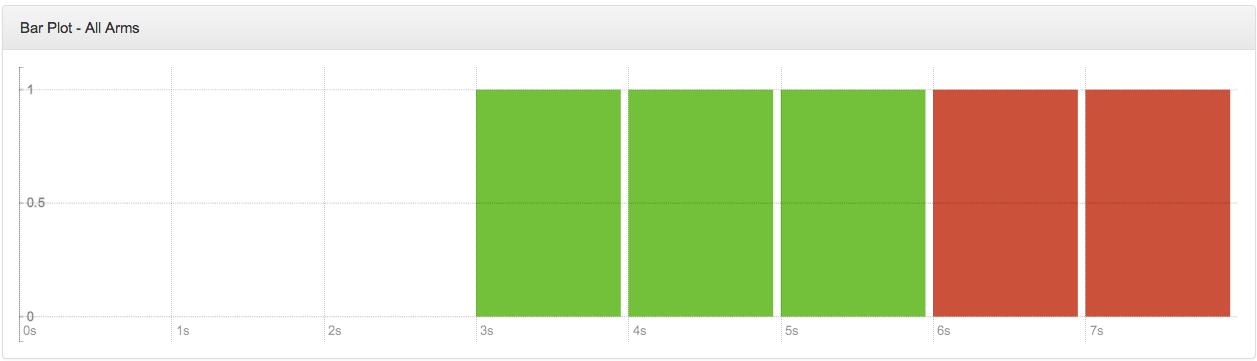
\includegraphics[scale=0.25]{barchart.png}
\end{frame}

\begin{frame}{File Upload - Line Chart}
\begin{itemize}
\item The line chart represents the average reward received over time
\item Each point on the line represents the number of times the arm was played divided by the total time elapsed
\end{itemize}
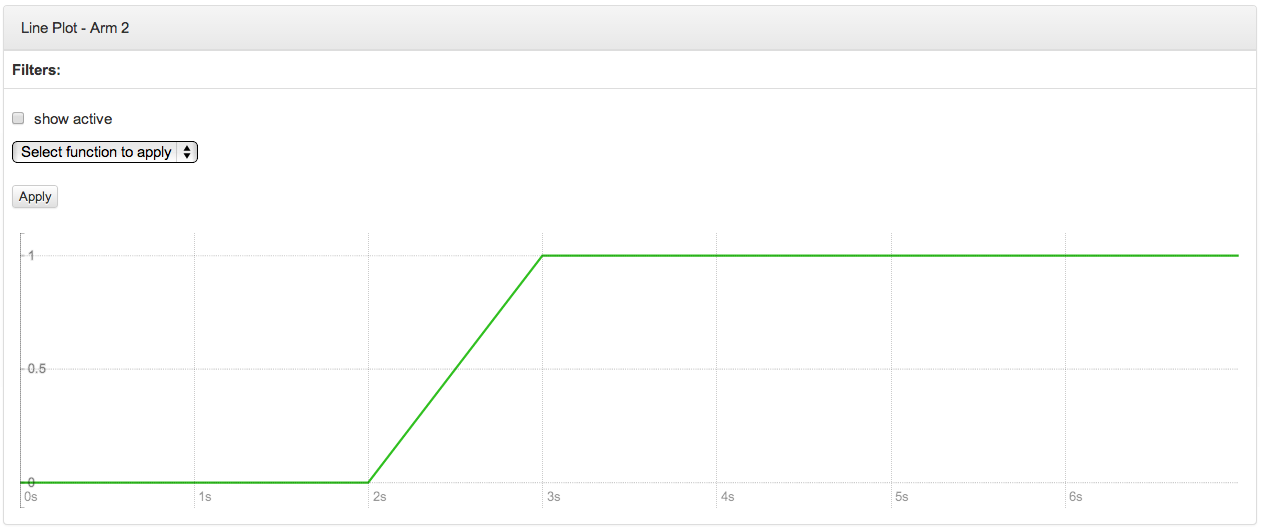
\includegraphics[scale=0.25]{linechart.png}
\end{frame}

\subsection{Arm Details}
\begin{frame}{Arm Details}
\begin{itemize}
\item Ability to differentiate between time arm was active/unactive
\end{itemize}
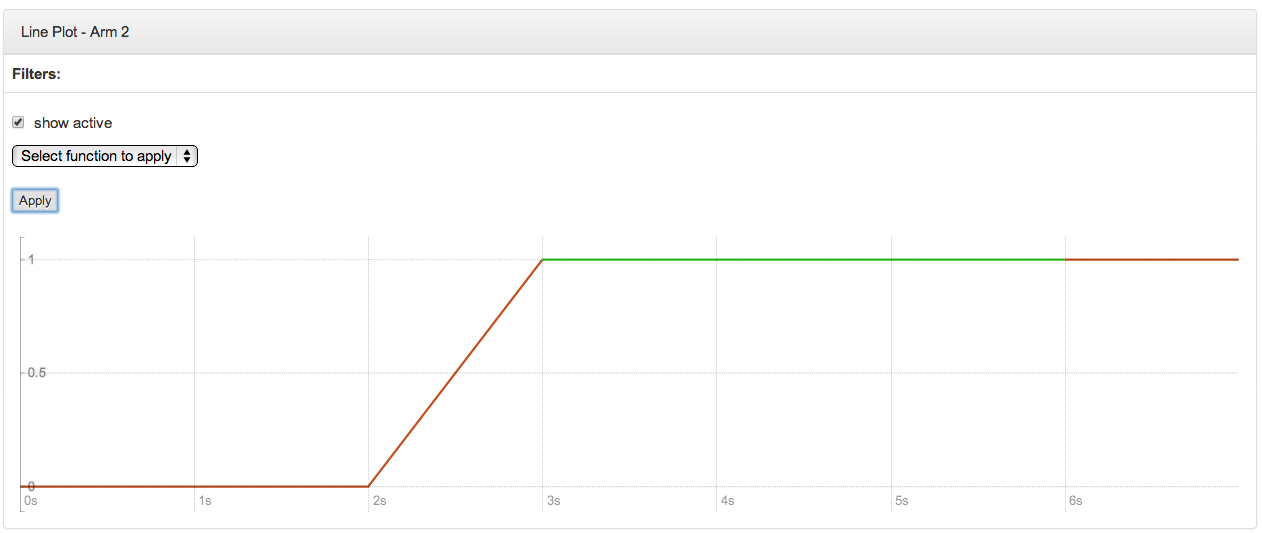
\includegraphics[scale=0.25]{linechartactive.png}
\end{frame}

\subsection{Viewing Results by Time}
\begin{frame}{Viewing Results by Time}
\begin{itemize}
\item For website optimization, traffic varies by time of day
\item In order to normalize time zones, bar chart displays results by hour
\end{itemize}
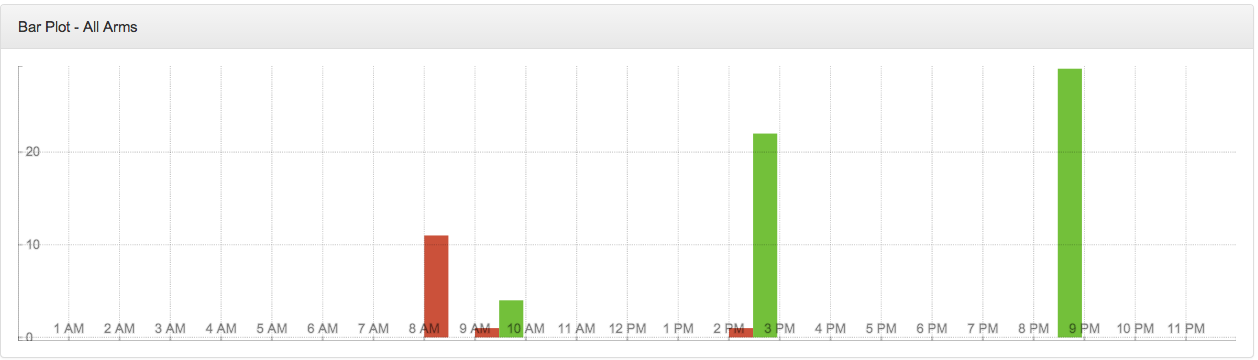
\includegraphics[scale=0.25]{barcharttime.png}
\end{frame}

\subsection{Applying a Function}
\begin{frame}{Applying a Function}
\begin{itemize}
\item Function is applied to the static data to generate a simulated line
\item Some functions include: UCB, Epsilon Greedy
\end{itemize}
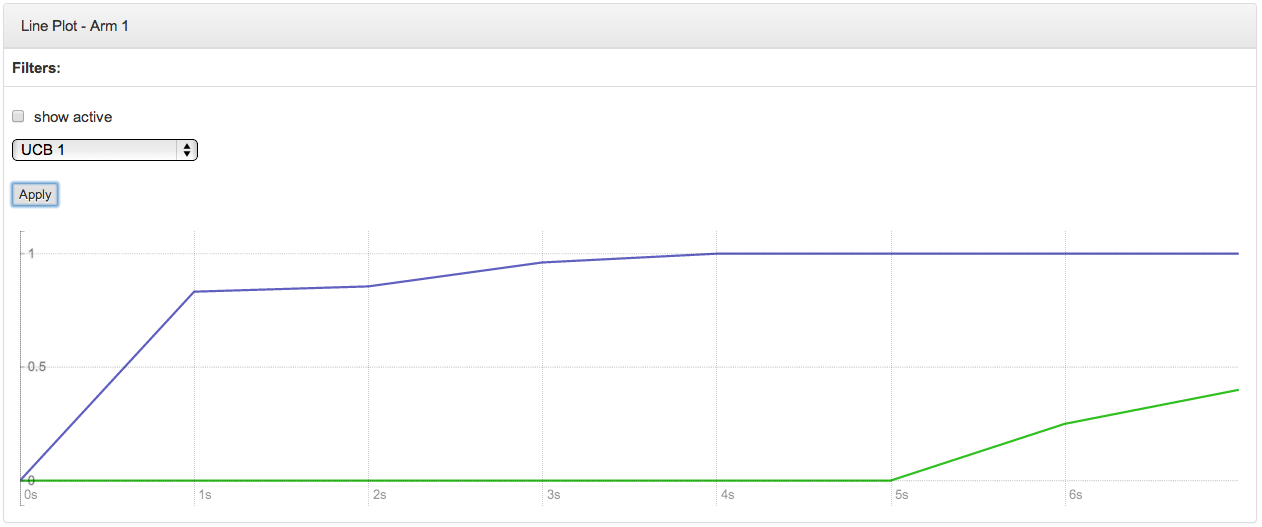
\includegraphics[scale=0.25]{linechartfunction.png}
\end{frame}

\section{Future Plans}

\subsection{Future Plans }
\begin{frame}{Support for Live Data and Enhanced Interactivity}
\begin{itemize}
\item Next major goal is to add support for live data
\item The application would listen to events sent by some client and produce graphs in realtime
\item The idea is to support multiple clients each having their own graphs
\item Increase in interactivity includes: hover effects, adding a slider to accomodate for large data and adding more filtering options
\item Define a common interface to communicate with the Web Application
\end{itemize}
\end{frame}


\section{Organization}

\subsection{Communication}
\begin{frame}{Communication}
\begin{itemize}
\item Primary forms of communication include: Email and Texts
\item Source code and documents are available on Dropbox
\item Tasks/Issues are created on GitHub so each member can easily pick a task and begin working on it
\item This is our backlog and new tasks will be added during each milestone
\item We aren't using any software process models like waterfall or agile
\end{itemize}
\end{frame}

\subsection{Issue Tracker}
\begin{frame}{Issue Tracker}
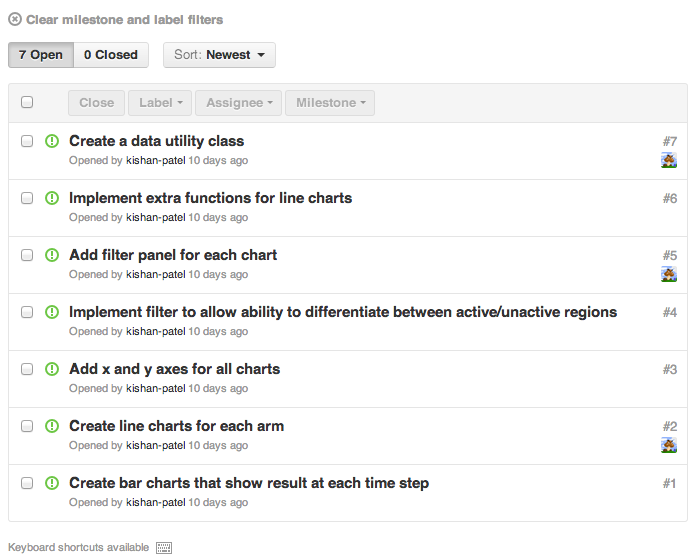
\includegraphics[scale=0.25]{gitissues.png}
\end{frame}

\subsection{Challenges}
\begin{frame}{Challenges}
\begin{itemize}
\item Testing will be challenging: We're not used to writing tests for web applications
\item Adding support for multiple clients and supporting live streaming is something that seems interesting as well as challenging
\item Finding a common schedule to work together
\end{itemize}
\end{frame}
\end{document}